
%% bare_jrnl.tex
%% V1.3
%% 2007/01/11
%% by Michael Shell
%% see http://www.michaelshell.org/
%% for current contact information.
%%
%% This is a skeleton file demonstrating the use of IEEEtran.cls
%% (requires IEEEtran.cls version 1.7 or later) with an IEEE journal paper.
%%
%% Support sites:
%% http://www.michaelshell.org/tex/ieeetran/
%% http://www.ctan.org/tex-archive/macros/latex/contrib/IEEEtran/
%% and
%% http://www.ieee.org/



% *** Authors should verify (and, if needed, correct) their LaTeX system  ***
% *** with the testflow diagnostic prior to trusting their LaTeX platform ***
% *** with production work. IEEE's font choices can trigger bugs that do  ***
% *** not appear when using other class files.                            ***
% The testflow support page is at:
% http://www.michaelshell.org/tex/testflow/


%%*************************************************************************
%% Legal Notice:
%% This code is offered as-is without any warranty either expressed or
%% implied; without even the implied warranty of MERCHANTABILITY or
%% FITNESS FOR A PARTICULAR PURPOSE! 
%% User assumes all risk.
%% In no event shall IEEE or any contributor to this code be liable for
%% any damages or losses, including, but not limited to, incidental,
%% consequential, or any other damages, resulting from the use or misuse
%% of any information contained here.
%%
%% All comments are the opinions of their respective authors and are not
%% necessarily endorsed by the IEEE.
%%
%% This work is distributed under the LaTeX Project Public License (LPPL)
%% ( http://www.latex-project.org/ ) version 1.3, and may be freely used,
%% distributed and modified. A copy of the LPPL, version 1.3, is included
%% in the base LaTeX documentation of all distributions of LaTeX released
%% 2003/12/01 or later.
%% Retain all contribution notices and credits.
%% ** Modified files should be clearly indicated as such, including  **
%% ** renaming them and changing author support contact information. **
%%
%% File list of work: IEEEtran.cls, IEEEtran_HOWTO.pdf, bare_adv.tex,
%%                    bare_conf.tex, bare_jrnl.tex, bare_jrnl_compsoc.tex
%%*************************************************************************

% Note that the a4paper option is mainly intended so that authors in
% countries using A4 can easily print to A4 and see how their papers will
% look in print - the typesetting of the document will not typically be
% affected with changes in paper size (but the bottom and side margins will).
% Use the testflow package mentioned above to verify correct handling of
% both paper sizes by the user's LaTeX system.
%
% Also note that the "draftcls" or "draftclsnofoot", not "draft", option
% should be used if it is desired that the figures are to be displayed in
% draft mode.
%
\documentclass[journal]{IEEEtran}
\usepackage{blindtext}
\usepackage{graphicx}
\usepackage{url}
\usepackage[utf8]{inputenc}

% Some very useful LaTeX packages include:
% (uncomment the ones you want to load)


% *** MISC UTILITY PACKAGES ***
%
%\usepackage{ifpdf}
% Heiko Oberdiek's ifpdf.sty is very useful if you need conditional
% compilation based on whether the output is pdf or dvi.
% usage:
% \ifpdf
%   % pdf code
% \else
%   % dvi code
% \fi
% The latest version of ifpdf.sty can be obtained from:
% http://www.ctan.org/tex-archive/macros/latex/contrib/oberdiek/
% Also, note that IEEEtran.cls V1.7 and later provides a builtin
% \ifCLASSINFOpdf conditional that works the same way.
% When switching from latex to pdflatex and vice-versa, the compiler may
% have to be run twice to clear warning/error messages.






% *** CITATION PACKAGES ***
%
%\usepackage{cite}
% cite.sty was written by Donald Arseneau
% V1.6 and later of IEEEtran pre-defines the format of the cite.sty package
% \cite{} output to follow that of IEEE. Loading the cite package will
% result in citation numbers being automatically sorted and properly
% "compressed/ranged". e.g., [1], [9], [2], [7], [5], [6] without using
% cite.sty will become [1], [2], [5]--[7], [9] using cite.sty. cite.sty's
% \cite will automatically add leading space, if needed. Use cite.sty's
% noadjust option (cite.sty V3.8 and later) if you want to turn this off.
% cite.sty is already installed on most LaTeX systems. Be sure and use
% version 4.0 (2003-05-27) and later if using hyperref.sty. cite.sty does
% not currently provide for hyperlinked citations.
% The latest version can be obtained at:
% http://www.ctan.org/tex-archive/macros/latex/contrib/cite/
% The documentation is contained in the cite.sty file itself.






% *** GRAPHICS RELATED PACKAGES ***
%
\ifCLASSINFOpdf
  % \usepackage[pdftex]{graphicx}
  % declare the path(s) where your graphic files are
  % \graphicspath{{../pdf/}{../jpeg/}}
  % and their extensions so you won't have to specify these with
  % every instance of \includegraphics
  % \DeclareGraphicsExtensions{.pdf,.jpeg,.png}
\else
  % or other class option (dvipsone, dvipdf, if not using dvips). graphicx
  % will default to the driver specified in the system graphics.cfg if no
  % driver is specified.
  % \usepackage[dvips]{graphicx}
  % declare the path(s) where your graphic files are
  % \graphicspath{{../eps/}}
  % and their extensions so you won't have to specify these with
  % every instance of \includegraphics
  % \DeclareGraphicsExtensions{.eps}
\fi
% graphicx was written by David Carlisle and Sebastian Rahtz. It is
% required if you want graphics, photos, etc. graphicx.sty is already
% installed on most LaTeX systems. The latest version and documentation can
% be obtained at: 
% http://www.ctan.org/tex-archive/macros/latex/required/graphics/
% Another good source of documentation is "Using Imported Graphics in
% LaTeX2e" by Keith Reckdahl which can be found as epslatex.ps or
% epslatex.pdf at: http://www.ctan.org/tex-archive/info/
%
% latex, and pdflatex in dvi mode, support graphics in encapsulated
% postscript (.eps) format. pdflatex in pdf mode supports graphics
% in .pdf, .jpeg, .png and .mps (metapost) formats. Users should ensure
% that all non-photo figures use a vector format (.eps, .pdf, .mps) and
% not a bitmapped formats (.jpeg, .png). IEEE frowns on bitmapped formats
% which can result in "jaggedy"/blurry rendering of lines and letters as
% well as large increases in file sizes.
%
% You can find documentation about the pdfTeX application at:
% http://www.tug.org/applications/pdftex





% *** MATH PACKAGES ***
%
%\usepackage[cmex10]{amsmath}
% A popular package from the American Mathematical Society that provides
% many useful and powerful commands for dealing with mathematics. If using
% it, be sure to load this package with the cmex10 option to ensure that
% only type 1 fonts will utilized at all point sizes. Without this option,
% it is possible that some math symbols, particularly those within
% footnotes, will be rendered in bitmap form which will result in a
% document that can not be IEEE Xplore compliant!
%
% Also, note that the amsmath package sets \interdisplaylinepenalty to 10000
% thus preventing page breaks from occurring within multiline equations. Use:
%\interdisplaylinepenalty=2500
% after loading amsmath to restore such page breaks as IEEEtran.cls normally
% does. amsmath.sty is already installed on most LaTeX systems. The latest
% version and documentation can be obtained at:
% http://www.ctan.org/tex-archive/macros/latex/required/amslatex/math/





% *** SPECIALIZED LIST PACKAGES ***
%
%\usepackage{algorithmic}
% algorithmic.sty was written by Peter Williams and Rogerio Brito.
% This package provides an algorithmic environment fo describing algorithms.
% You can use the algorithmic environment in-text or within a figure
% environment to provide for a floating algorithm. Do NOT use the algorithm
% floating environment provided by algorithm.sty (by the same authors) or
% algorithm2e.sty (by Christophe Fiorio) as IEEE does not use dedicated
% algorithm float types and packages that provide these will not provide
% correct IEEE style captions. The latest version and documentation of
% algorithmic.sty can be obtained at:
% http://www.ctan.org/tex-archive/macros/latex/contrib/algorithms/
% There is also a support site at:
% http://algorithms.berlios.de/index.html
% Also of interest may be the (relatively newer and more customizable)
% algorithmicx.sty package by Szasz Janos:
% http://www.ctan.org/tex-archive/macros/latex/contrib/algorithmicx/




% *** ALIGNMENT PACKAGES ***
%
%\usepackage{array}
% Frank Mittelbach's and David Carlisle's array.sty patches and improves
% the standard LaTeX2e array and tabular environments to provide better
% appearance and additional user controls. As the default LaTeX2e table
% generation code is lacking to the point of almost being broken with
% respect to the quality of the end results, all users are strongly
% advised to use an enhanced (at the very least that provided by array.sty)
% set of table tools. array.sty is already installed on most systems. The
% latest version and documentation can be obtained at:
% http://www.ctan.org/tex-archive/macros/latex/required/tools/


%\usepackage{mdwmath}
%\usepackage{mdwtab}
% Also highly recommended is Mark Wooding's extremely powerful MDW tools,
% especially mdwmath.sty and mdwtab.sty which are used to format equations
% and tables, respectively. The MDWtools set is already installed on most
% LaTeX systems. The lastest version and documentation is available at:
% http://www.ctan.org/tex-archive/macros/latex/contrib/mdwtools/


% IEEEtran contains the IEEEeqnarray family of commands that can be used to
% generate multiline equations as well as matrices, tables, etc., of high
% quality.


%\usepackage{eqparbox}
% Also of notable interest is Scott Pakin's eqparbox package for creating
% (automatically sized) equal width boxes - aka "natural width parboxes".
% Available at:
% http://www.ctan.org/tex-archive/macros/latex/contrib/eqparbox/





% *** SUBFIGURE PACKAGES ***
%\usepackage[tight,footnotesize]{subfigure}
% subfigure.sty was written by Steven Douglas Cochran. This package makes it
% easy to put subfigures in your figures. e.g., "Figure 1a and 1b". For IEEE
% work, it is a good idea to load it with the tight package option to reduce
% the amount of white space around the subfigures. subfigure.sty is already
% installed on most LaTeX systems. The latest version and documentation can
% be obtained at:
% http://www.ctan.org/tex-archive/obsolete/macros/latex/contrib/subfigure/
% subfigure.sty has been superceeded by subfig.sty.



%\usepackage[caption=false]{caption}
%\usepackage[font=footnotesize]{subfig}
% subfig.sty, also written by Steven Douglas Cochran, is the modern
% replacement for subfigure.sty. However, subfig.sty requires and
% automatically loads Axel Sommerfeldt's caption.sty which will override
% IEEEtran.cls handling of captions and this will result in nonIEEE style
% figure/table captions. To prevent this problem, be sure and preload
% caption.sty with its "caption=false" package option. This is will preserve
% IEEEtran.cls handing of captions. Version 1.3 (2005/06/28) and later 
% (recommended due to many improvements over 1.2) of subfig.sty supports
% the caption=false option directly:
%\usepackage[caption=false,font=footnotesize]{subfig}
%
% The latest version and documentation can be obtained at:
% http://www.ctan.org/tex-archive/macros/latex/contrib/subfig/
% The latest version and documentation of caption.sty can be obtained at:
% http://www.ctan.org/tex-archive/macros/latex/contrib/caption/




% *** FLOAT PACKAGES ***
%
%\usepackage{fixltx2e}
% fixltx2e, the successor to the earlier fix2col.sty, was written by
% Frank Mittelbach and David Carlisle. This package corrects a few problems
% in the LaTeX2e kernel, the most notable of which is that in current
% LaTeX2e releases, the ordering of single and double column floats is not
% guaranteed to be preserved. Thus, an unpatched LaTeX2e can allow a
% single column figure to be placed prior to an earlier double column
% figure. The latest version and documentation can be found at:
% http://www.ctan.org/tex-archive/macros/latex/base/



%\usepackage{stfloats}
% stfloats.sty was written by Sigitas Tolusis. This package gives LaTeX2e
% the ability to do double column floats at the bottom of the page as well
% as the top. (e.g., "\begin{figure*}[!b]" is not normally possible in
% LaTeX2e). It also provides a command:
%\fnbelowfloat
% to enable the placement of footnotes below bottom floats (the standard
% LaTeX2e kernel puts them above bottom floats). This is an invasive package
% which rewrites many portions of the LaTeX2e float routines. It may not work
% with other packages that modify the LaTeX2e float routines. The latest
% version and documentation can be obtained at:
% http://www.ctan.org/tex-archive/macros/latex/contrib/sttools/
% Documentation is contained in the stfloats.sty comments as well as in the
% presfull.pdf file. Do not use the stfloats baselinefloat ability as IEEE
% does not allow \baselineskip to stretch. Authors submitting work to the
% IEEE should note that IEEE rarely uses double column equations and
% that authors should try to avoid such use. Do not be tempted to use the
% cuted.sty or midfloat.sty packages (also by Sigitas Tolusis) as IEEE does
% not format its papers in such ways.


%\ifCLASSOPTIONcaptionsoff
%  \usepackage[nomarkers]{endfloat}
% \let\MYoriglatexcaption\caption
% \renewcommand{\caption}[2][\relax]{\MYoriglatexcaption[#2]{#2}}
%\fi
% endfloat.sty was written by James Darrell McCauley and Jeff Goldberg.
% This package may be useful when used in conjunction with IEEEtran.cls'
% captionsoff option. Some IEEE journals/societies require that submissions
% have lists of figures/tables at the end of the paper and that
% figures/tables without any captions are placed on a page by themselves at
% the end of the document. If needed, the draftcls IEEEtran class option or
% \CLASSINPUTbaselinestretch interface can be used to increase the line
% spacing as well. Be sure and use the nomarkers option of endfloat to
% prevent endfloat from "marking" where the figures would have been placed
% in the text. The two hack lines of code above are a slight modification of
% that suggested by in the endfloat docs (section 8.3.1) to ensure that
% the full captions always appear in the list of figures/tables - even if
% the user used the short optional argument of \caption[]{}.
% IEEE papers do not typically make use of \caption[]'s optional argument,
% so this should not be an issue. A similar trick can be used to disable
% captions of packages such as subfig.sty that lack options to turn off
% the subcaptions:
% For subfig.sty:
% \let\MYorigsubfloat\subfloat
% \renewcommand{\subfloat}[2][\relax]{\MYorigsubfloat[]{#2}}
% For subfigure.sty:
% \let\MYorigsubfigure\subfigure
% \renewcommand{\subfigure}[2][\relax]{\MYorigsubfigure[]{#2}}
% However, the above trick will not work if both optional arguments of
% the \subfloat/subfig command are used. Furthermore, there needs to be a
% description of each subfigure *somewhere* and endfloat does not add
% subfigure captions to its list of figures. Thus, the best approach is to
% avoid the use of subfigure captions (many IEEE journals avoid them anyway)
% and instead reference/explain all the subfigures within the main caption.
% The latest version of endfloat.sty and its documentation can obtained at:
% http://www.ctan.org/tex-archive/macros/latex/contrib/endfloat/
%
% The IEEEtran \ifCLASSOPTIONcaptionsoff conditional can also be used
% later in the document, say, to conditionally put the References on a 
% page by themselves.





% *** PDF, URL AND HYPERLINK PACKAGES ***
%
%\usepackage{url}
% url.sty was written by Donald Arseneau. It provides better support for
% handling and breaking URLs. url.sty is already installed on most LaTeX
% systems. The latest version can be obtained at:
% http://www.ctan.org/tex-archive/macros/latex/contrib/misc/
% Read the url.sty source comments for usage information. Basically,
% \url{my_url_here}.





% *** Do not adjust lengths that control margins, column widths, etc. ***
% *** Do not use packages that alter fonts (such as pslatex).         ***
% There should be no need to do such things with IEEEtran.cls V1.6 and later.
% (Unless specifically asked to do so by the journal or conference you plan
% to submit to, of course. )


% correct bad hyphenation here
\hyphenation{op-tical net-works semi-conduc-tor}
\usepackage{authblk}
\usepackage{graphicx}


\begin{document}
%
% paper title
% can use linebreaks \\ within to get better formatting as desired
\title {Mapping Unsustainable Health and Sanitation practices at the Pashmina Weaving Unit in Shankarpur Village }
%
%
% author names and IEEE memberships
% note positions of commas and nonbreaking spaces ( ~ ) LaTeX will not break
% a structure at a ~ so this keeps an author's name from being broken across
% two lines.
% use \thanks{} to gain access to the first footnote area
% a separate \thanks must be used for each paragraph as LaTeX2e's \thanks
% was not built to handle multiple paragraphs
%

\author[1]{Anwesh Kumar Sahoo}
\author[1]{Swati Mishra, ~\IEEEmembership{Master of Design,} \\{\small Advisor: Dr. Varsha Gupta}}

       

\affil{National Institute of Fashion Technology, New Delhi}
\date{25 April}
      % <-this % stops a space
%\thanks{M. Shell is with the Department
%of Electrical and Computer Engineering, Georgia Institute of Technology, Atlanta,
%GA, 30332 USA e-mail: (see http://www.michaelshell.org/contact.html).}% <-this % stops a space
%\thanks{J. Doe and J. Doe are with Anonymous University.}% <-this % stops a space
%\thanks{Manuscript received April 19, 2005; revised January 11, 2007.}}


% note the % following the last \IEEEmembership and also \thanks - 
% these prevent an unwanted space from occurring between the last author name
% and the end of the author line. i.e., if you had this:
% 
% \author{....lastname \thanks{...} \thanks{...} }
%                     ^------------^------------^----Do not want these spaces!
%
% a space would be appended to the last name and could cause every name on that
% line to be shifted left slightly. This is one of those "LaTeX things". For
% instance, "\textbf{A} \textbf{B}" will typeset as "A B" not "AB". To get
% "AB" then you have to do: "\textbf{A}\textbf{B}"
% \thanks is no different in this regard, so shield the last } of each \thanks
% that ends a line with a % and do not let a space in before the next \thanks.
% Spaces after \IEEEmembership other than the last one are OK (and needed) as
% you are supposed to have spaces between the names. For what it is worth,
% this is a minor point as most people would not even notice if the said evil
% space somehow managed to creep in.



% The paper headers
%\markboth{Journal of \LaTeX\ Class Files,~Vol.~6, No.~1, January~2007}

% The only time the second header will appear is for the odd numbered pages
% after the title page when using the twoside option.
% 
% *** Note that you probably will NOT want to include the author's ***
% *** name in the headers of peer review papers.                   ***
% You can use \ifCLASSOPTIONpeerreview for conditional compilation here if
% you desire.




% If you want to put a publisher's ID mark on the page you can do it like
% this:
%\IEEEpubid{0000--0000/00\$00.00~\copyright~2007 IEEE}
% Remember, if you use this you must call \IEEEpubidadjcol in the second
% column for its text to clear the IEEEpubid mark.



% use for special paper notices
%\IEEEspecialpapernotice{(Invited Paper)}




% make the title area
\maketitle

\begin{abstract}
    \textit{Pashmina}, also popularly known as Cashmere is well known for its softness, fineness, and the sky high prices at which \textit{pashmina} based shawls and scarves are sold. Behind these exquisite shawls are the weavers who work day in, and day out to make their ends meet. A weaving unit in Shankarpur village in Rampur, is one such unit involved in the weaving of \textit{pashmina}, shawls, scarves and even saris. This is a well established fact that a major percentage of individuals in India are yet to have access to adequate facilities for waste disposal, defecation, and awareness related to fundamental health and sanitation practices, especially at their work spaces. In a weaving unit like the one we visited to, an absence of a well defined schedule sometimes adversely affects the kids of the parents involved in the weaving, and production. An attempt has been made to provide a comprehensive review covering the various unsustainable practices that were observed keeping the health and fundamental sanitation of the artists in mind. Solutions to the existing issues have also been listed which could be adopted by the unit, to ensure a healthy sustainable functioning of both the lives of the artisans, and the weaving unit in the long run.
\end{abstract}
 


% IEEEtran.cls defaults to using nonbold math in the Abstract.
% This preserves the distinction between vectors and scalars. However,
% if the journal you are submitting to favors bold math in the abstract,
% then you can use LaTeX's standard command \boldmath at the very start
% of the abstract to achieve this. Many IEEE journals frown on math
% in the abstract anyway.

% Note that keywords are not normally used for peerreview papers.
\begin{IEEEkeywords}
Pashmina, Cashmere, Health and Sanitation, Dehairing, Fibre, Shawl, Wool. 
\end{IEEEkeywords}






% For peer review papers, you can put extra information on the cover
% page as needed:
% \ifCLASSOPTIONpeerreview
% \begin{center} \bfseries EDICS Category: 3-BBND \end{center}
% \fi
%
% For peerreview papers, this IEEEtran command inserts a page break and
% creates the second title. It will be ignored for other modes.
\IEEEpeerreviewmaketitle


\section{Introduction}
The Indian weaving industry has conventionally been one of the most promising sectors, creating massive employment opportunities over the years. The Indian textiles industry is extremely varied, with the hand-spun and hand-woven textiles sectors at one end of the spectrum, while the capital intensive sophisticated mills sector at the other end of the spectrum. with such a wide spectrum and varied heritage, it is still lagging in some fields that are making it unsustainable. Occupational hazards, health issues, hygiene and sanitation, paucity of maternity care, lack of infrastructure are to name a few. The hazards can be divided into two broad categories- Environmental hazards and, Physical hazards. We cover the above mentioned topics in detail through the course of this paper, with a map of the system, suggesting ways in which the system could be made more sustainable, ensuring quality life for the weavers and artisans. 


\section{Impact of scarcity of light on vision:}
Speaking to Md. Iliyas ji, the Master craftsman who is well into his 70s, we were exposed to issues he was dealing with related to his gradual loss in clear vision. While he stated it was related to his aging, which could be partially true, we were drawn to another factor that could possibly be affecting the vision of all the artisans working under the Cluster. One of them was the paucity of ambient light in the workshop. Iliyas ji believed in working throughout the day till dusk. While there were small bulbs attached to the ceiling, they didn’t believe in using the same while at work. The bulbs were only used when the work had to be done overnight to meet mounting deadlines, which is seldom a situation. 

\par 
Lighting and mental acuity are closely related. Although dim lighting will not adversely affect one’s eyesight, it will tire one’s eyes out more quickly. Working in an area with dim lighting, can also make one less productive, and can make one find it difficult to sleep at night.  According to a study conducted by Michigan State University, working under dim-light conditions can lead to a fall in the production of a certain peptide in the brain responsible for maintaining the connection between neurons in the hippocampus of the brain. As quoted by Antonio Nunez, a psychology professor and co- investigator on the study, “Since there are fewer connections being made, this results in diminished learning and memory performance that is dependent upon the hippocampus. In other words, dim lights are producing dimwits.” 
\par 
Another condition called Macular Degeneration, an eye disorder that affects the retina, the light-sensitive area where images are formed, is primarily caused by age. Vision loss can also be caused by a hereditary form of macular degeneration. The condition also leads to reading difficulties, a symptom which was also seen in Iliyas ji. Age-related macular generation is most commonly referred to as non-exudative, or the dry form in which visiaol loss is mostly gradual. This condition is further worsened with paucity of ambient light while reading or working. Iliyas ji is often seen working on the charka now, and dim-lighting conditions are certainly not making it any better for him to function.



 

\section{Back and Joint related issues owing to incorrect Posture}

 A part of chiropractic philosophy deals with how subluxations in one’s spine can impact one’s entire body, and not just the the back, and the joints. This is one of the major reasons why chiropractic care in conjugation with one’s mindfulness is vital. The female members of the family often spends hours working on the charka, often working for hours together without a break, and are most prone to joint and back related issues. First off, poor posture can impact one’s lung’s functioning.

\par
\subsection{Lung Function}
\par Poor postures can impact the amount of air inhaled by an individual when one breathes. Therefore, hunching forward, or leaning can negatively influence one’s lungs’ functioning.  how much air you can take into your lungs when you breathe. This means that when our lungs don’t function to their highest potential, our heart, our brain, and our vital organs get affected in the process, given adequate oxygen doesn’t reach our system. This in turn shortness of breath, as well as poor cognitive abilities. Sometimes, even worse; cardiovascular diseases.

\subsection{Back and Shoulder Pain}
\par One of the most common effects of bad posture is chronic back pain, simply because of the excess pressure suffered by the spine, or even due to disc degeneration which is when the disks between the vertebrae thin out, and lose their cushioning. Slouching can even lead to tension in the upper back, shoulders and even a permanent hump. When one pulls one’s shoulders way too far back, the same can cause the muscles to tense, and even lead to stiffness. 



\begin{figure}
  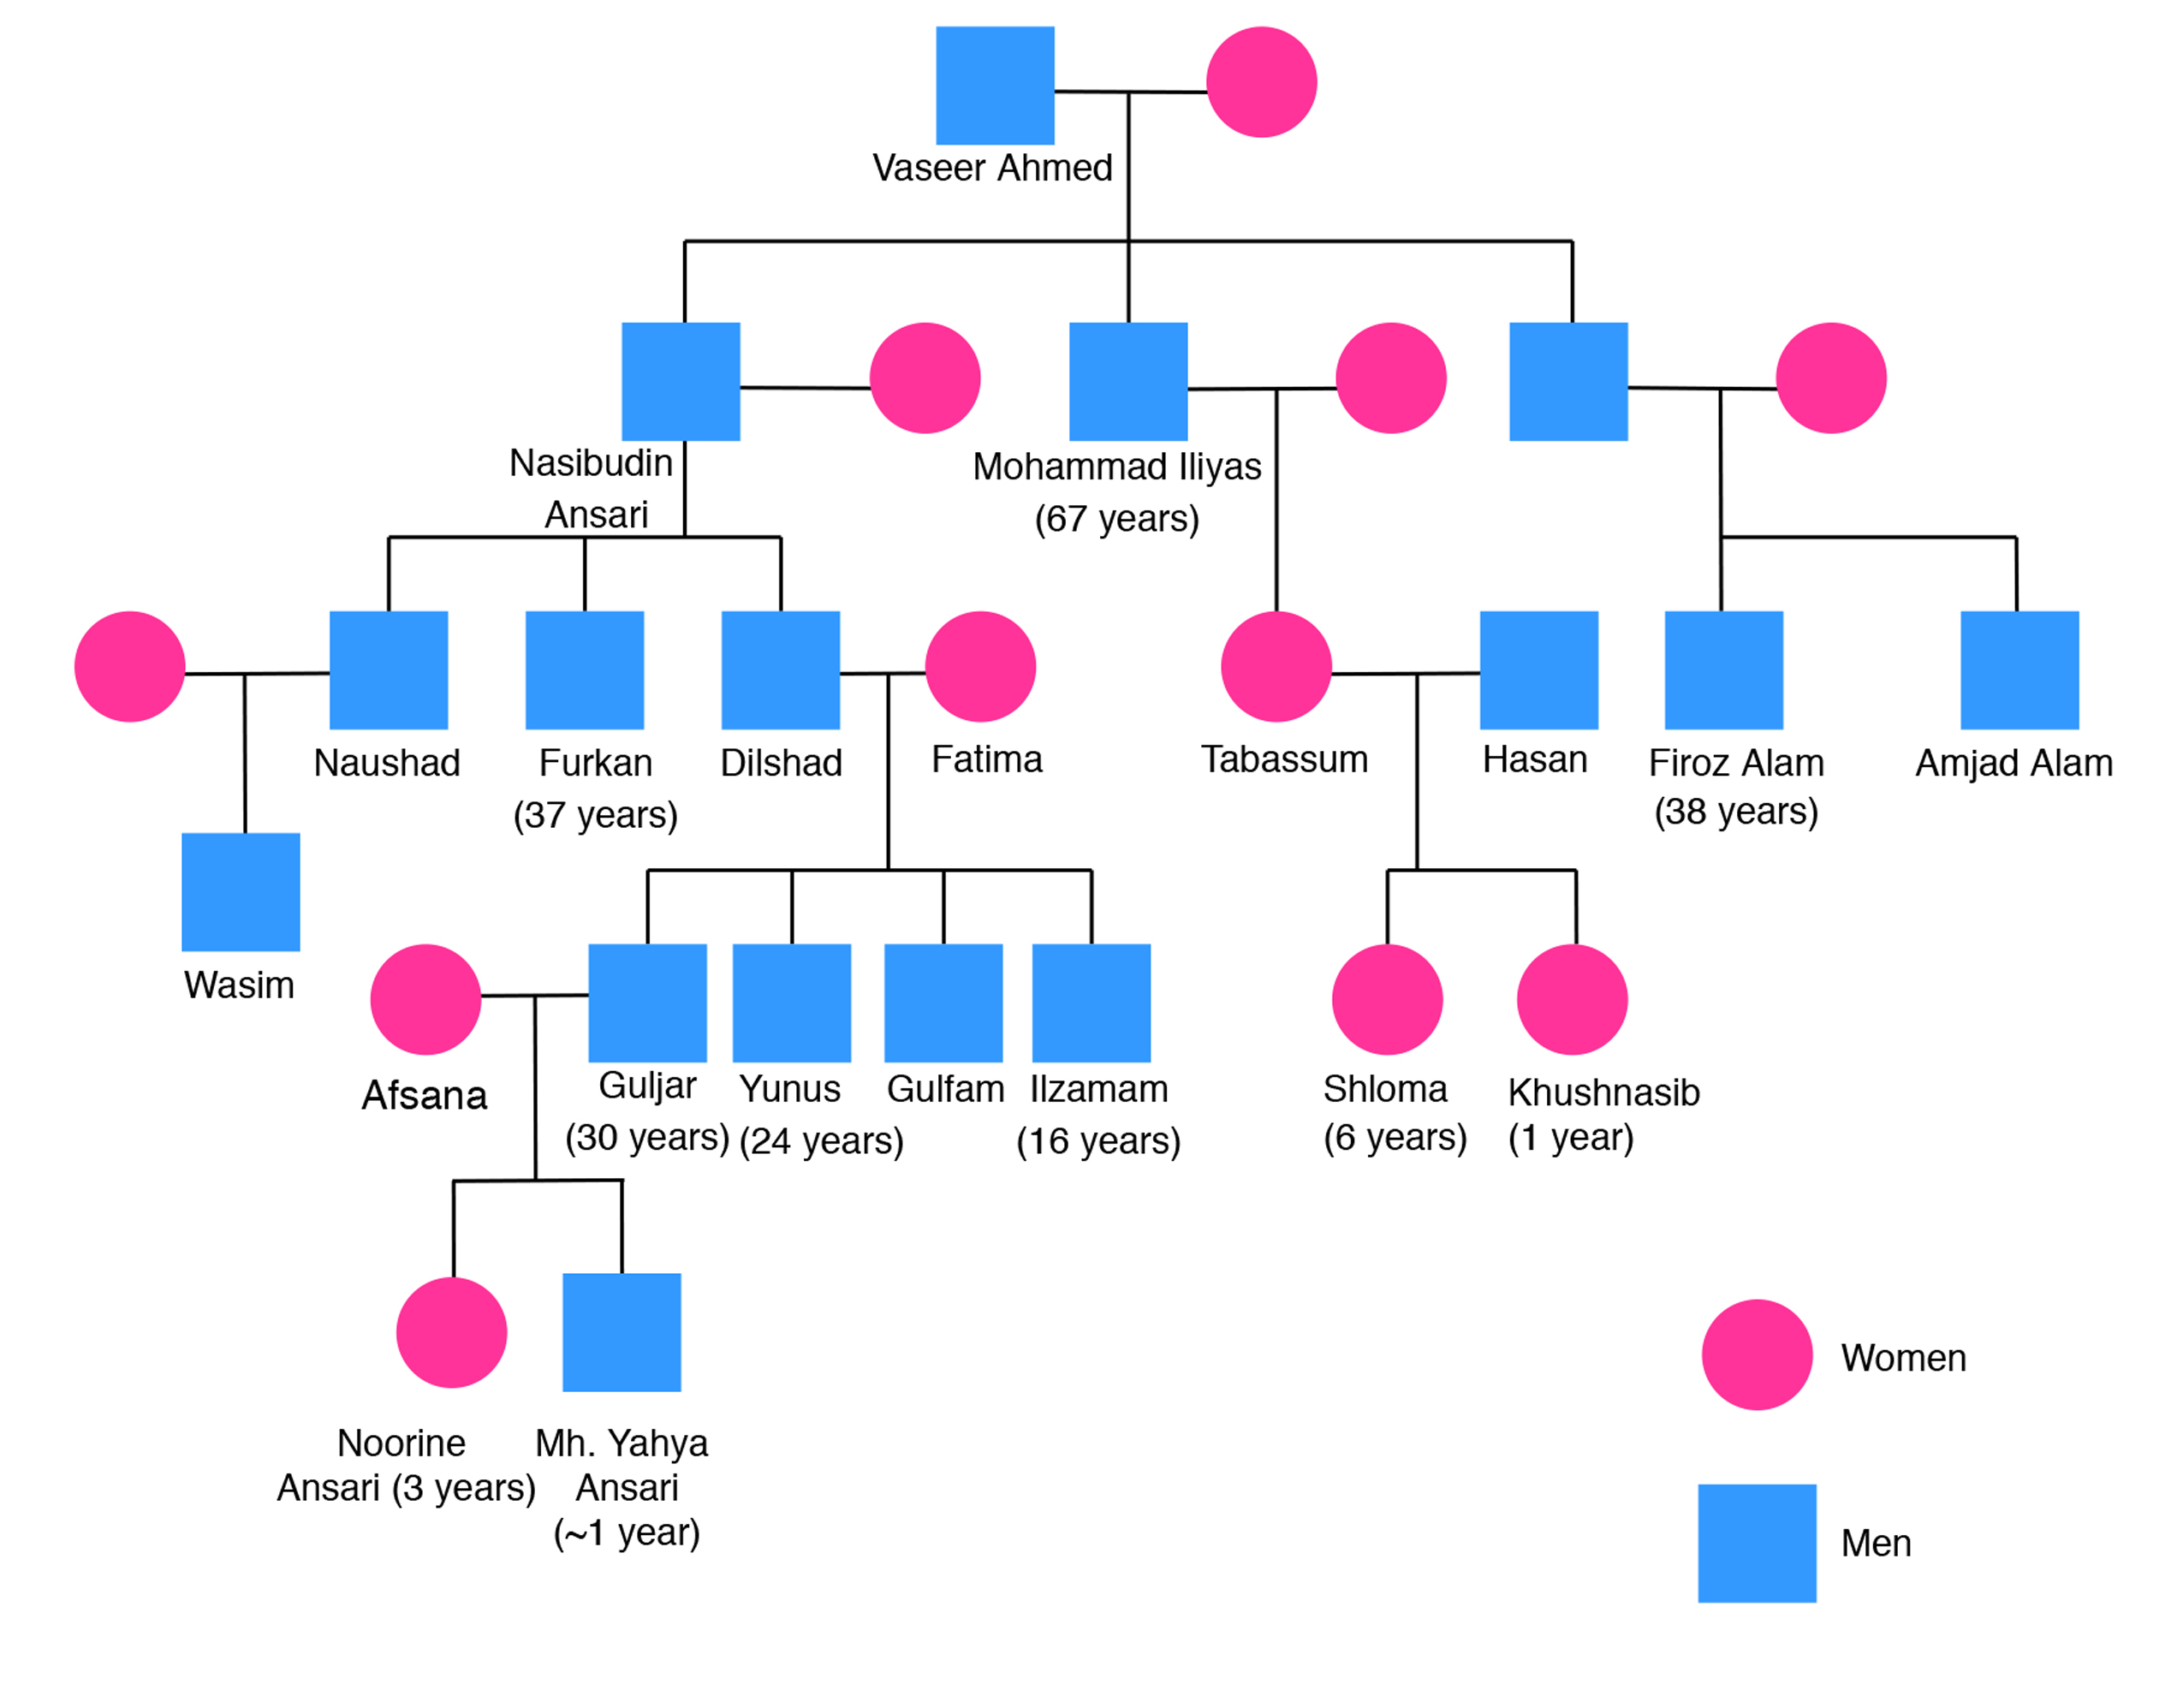
\includegraphics[width=\linewidth]{tree1.jpg}
  \caption{Family Tree of Pashmina Weavers at Shankarpur Village}
  \label{Family Tree Pashmina Cluster}
\end{figure}




\section{Paucity of time dedicated to kids}
Spending time with the artisans, and discussing their schedule also made us take a peek into a day in their lives. It was pretty apparent that the artisans lacked a defined schedule in the entire day. While they all woke up early and started working at the workshop at around 7:30-8 in the morning, their work spanned the entire day till dusk, with no defined time for a break. The mother Tabassum ji (the family tree can be dotted via figure 1), with two little daughters, and a third child on its way hardly had any time in hand to spare for her youngest daughter who was 10 months old. She was unable to keep a check on what Khushnaseeb would eat for instance, and was often seen with a small packet of junk food to make her stop crying. The mother was the only one who was expected to take care of the babies, with Iliyas ji (their grandfather) pitching in only a few times, until she’d start crying again. The elder daughter too was unable to have her mother by her side, especially while she was getting ready for school. She didn’t have much guidance once she was back from school either. The other female members of the family, were either involved on the charka, or mostly involved in household chores. Allocation of well defined duties for all the artisans involved in their respective duties, with a fixed schedule was still a concern which made it relatively difficult for especially women to balance both their work at home as well as at their work. 



\section{ Lack of fundamental sanitation}
At our time of visit to the workshop, there were only 6 artisans in total at the weaving unit, with one female artisan, Tabassum ji. Tabassum ji and her family, along with Md. Iliyas ji also shared their personal space/home with the weaving unit. However, there was only one washroom available, with a barely there fabric just covering the opening of the bathing space. The washroom was dirty, with a flimsy door covering the opening. There was a clear lack of basic hygiene levels, and almost no privacy for the female artisan. The family members, children, and the artisans working at the unit had to all use the same space for defecation. The clothes of the family members were being used at the same space, in a pool of water and dirt, and a thick growth of algae on the wall. In fact the entire staircase built just next to the bathing area was filled with algae, and was extremely flimsy, posing a threat for the kids who ran . The pipes put inside the washrooms, had an outlet just outside the house in the backyard, with an absence of a drainage system. 

Another aspect which was neglected was the presence of multiple mongooses around the workshop, and the absence of doors around the house, would make it easier for snakes and rodents to crawl/walk into the workshop. The children, especially the infants were at the highest risk of being bitten. To add to that since there was no one actively present to take care of the kids, the infants were seen eating food, and dirt off the floor, putting them at risk of infections. 

\begin{figure}
  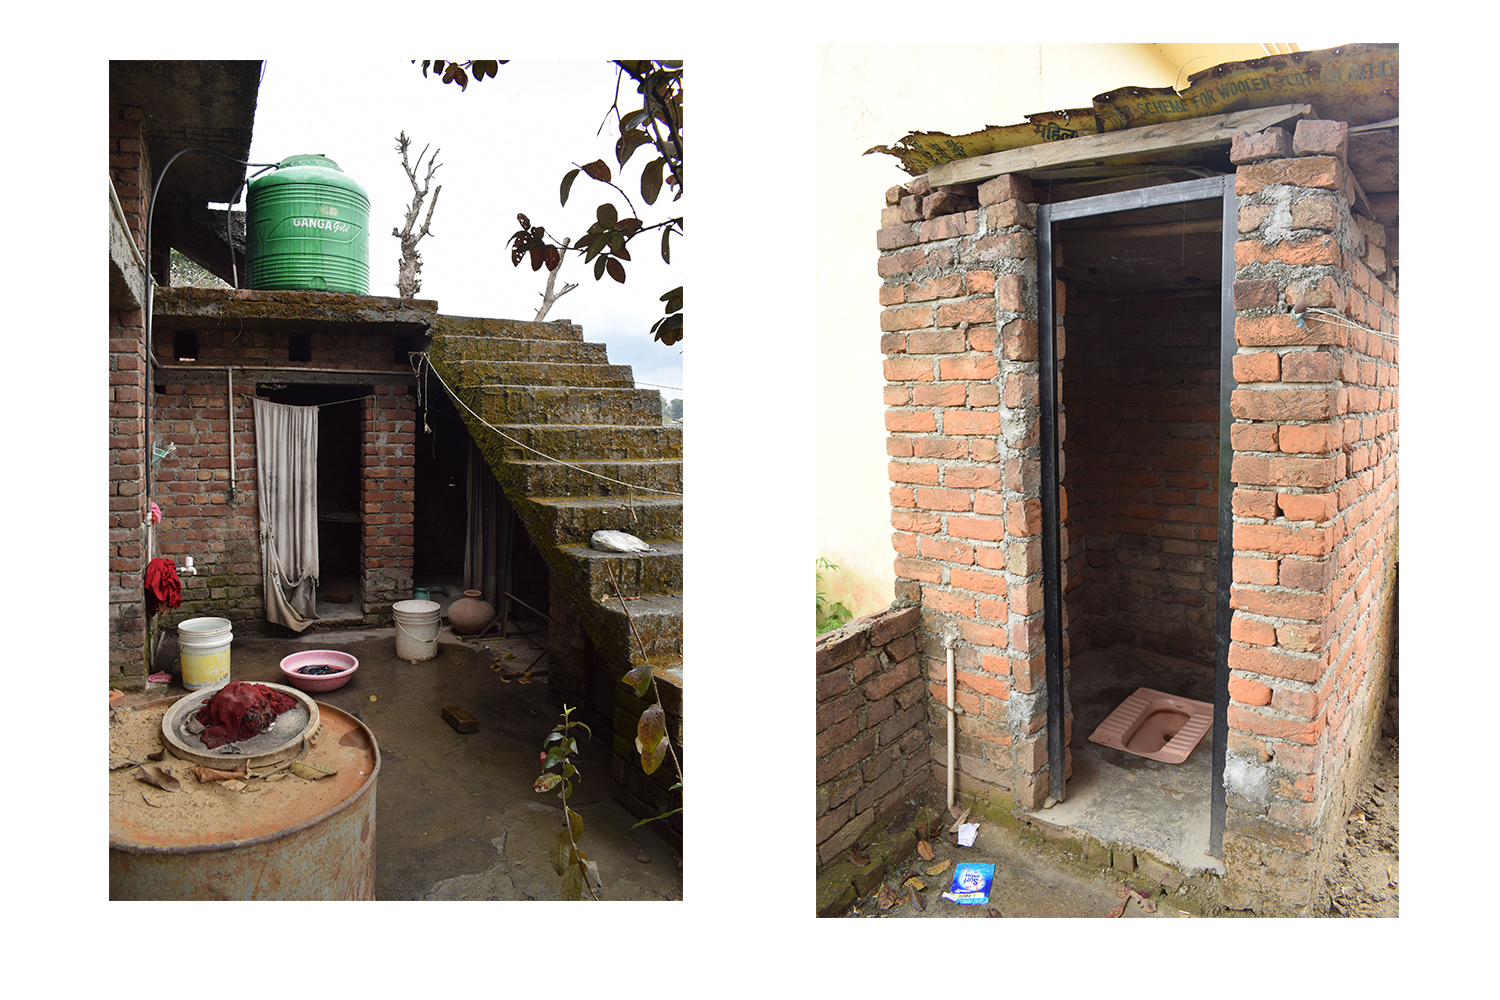
\includegraphics[width=\linewidth]{toilet.jpg}
  \caption{The washroom without a door at the weaving unit (self-clicked)}
  \label{Family Tree Pashmina Cluster}
\end{figure}

\section{Fibre pollution at weaving unit owing to wool and carding (Dunda)
} 

\subsection{Occupational health hazard}
Diseases or health issues occurred due to exposure within the work place is called as occupational health hazards. 

In india, Due to lack of education, lack of awareness about the hazards of their occupations, poor  sanitation, poor nutrition and unorganized sector the occupational health hazards increase.


\subsection{Respiratory diseases}

There are various disciplines which are related to Occupational Health and Safety like epidemiology, industrial hygiene, occupational nursing, toxicology etc. It involves the conditions and surroundings that influence workers at working environment. Occupational health and safety practices is the large concern for the protection from hazards at the workplace. Among various health hazards,  the fibre dust pollution is a major concern for textile workers.

\par 
A survey was conducted in 2011 at The Bhadohi Textile Corporation Limited, which has three textile mills. It included all female employees, in the 20-49 years of age group, who had been working in the factory for at least more than 3 months. 
The analysis was done for 243 subjects- 57 from the spinning section, 32 from
the scouring section, 65 from the weaving section, 89 from the non-dusty sections and 235 non textile workers working in different industries or working in farm field, or acting as housewives. The present research paper (titled, 'A study of the occupational health function among female textile workers', 2011) maps 95 cases of respiratory problems found in the case of Textile workers, but in the case of Non-Textile workers only 15 cases were found, of whom 28 had associated chest pain with cough. For the risk factor analysis, 67 cases with only symptomatic respiratory problems were included (via, 'A study of the occupational health function among female textile workers, 2011') 

\par
The results showed that workers in the scouring section had 11.0 times, spinning section had 4.7 times and those in the weaving section had 2.6 times higher risk of developing respiratory problems compared with those working in the non-dusty sections.

\par
Some of the effects of the fibre dust are listed as follows: 
\begin{itemize}
    \item Formation of fibre film on surfaces 
    \item Particles fall into moving parts of machinery
    \item Dirty appearance of product
\end{itemize}

\subsection{Byssinosis - an occupational Health Hazard}

\par
Byssinosis is an occupational lung disease. It affects workers in cotton, wool processing, and hemp or flax industries. Other names for byssinosis include Monday fever, brown lung disease, mill fever or cotton workers' lung.

Some of the major symptoms of Byssinosis are as follows:
\begin{itemize}
    \item Cough
    \item Difficulty in breathing
    \item Chest tightness
    \item Shivering
    \item Flu-like muscle pain
    \item Joint pain
    \item Tiredness
    \item Dry cough
    \item Shortness of breath
\end{itemize}

\par
Some of the common ways of treatment are listed below:
\begin{itemize}
    \item Consider alternate occupation (in severe cases)
    \item Physical exercises and breathing exercises might help
    \item Other symptomatic treatment and, supportive therapy
\end{itemize}

\begin{figure}
  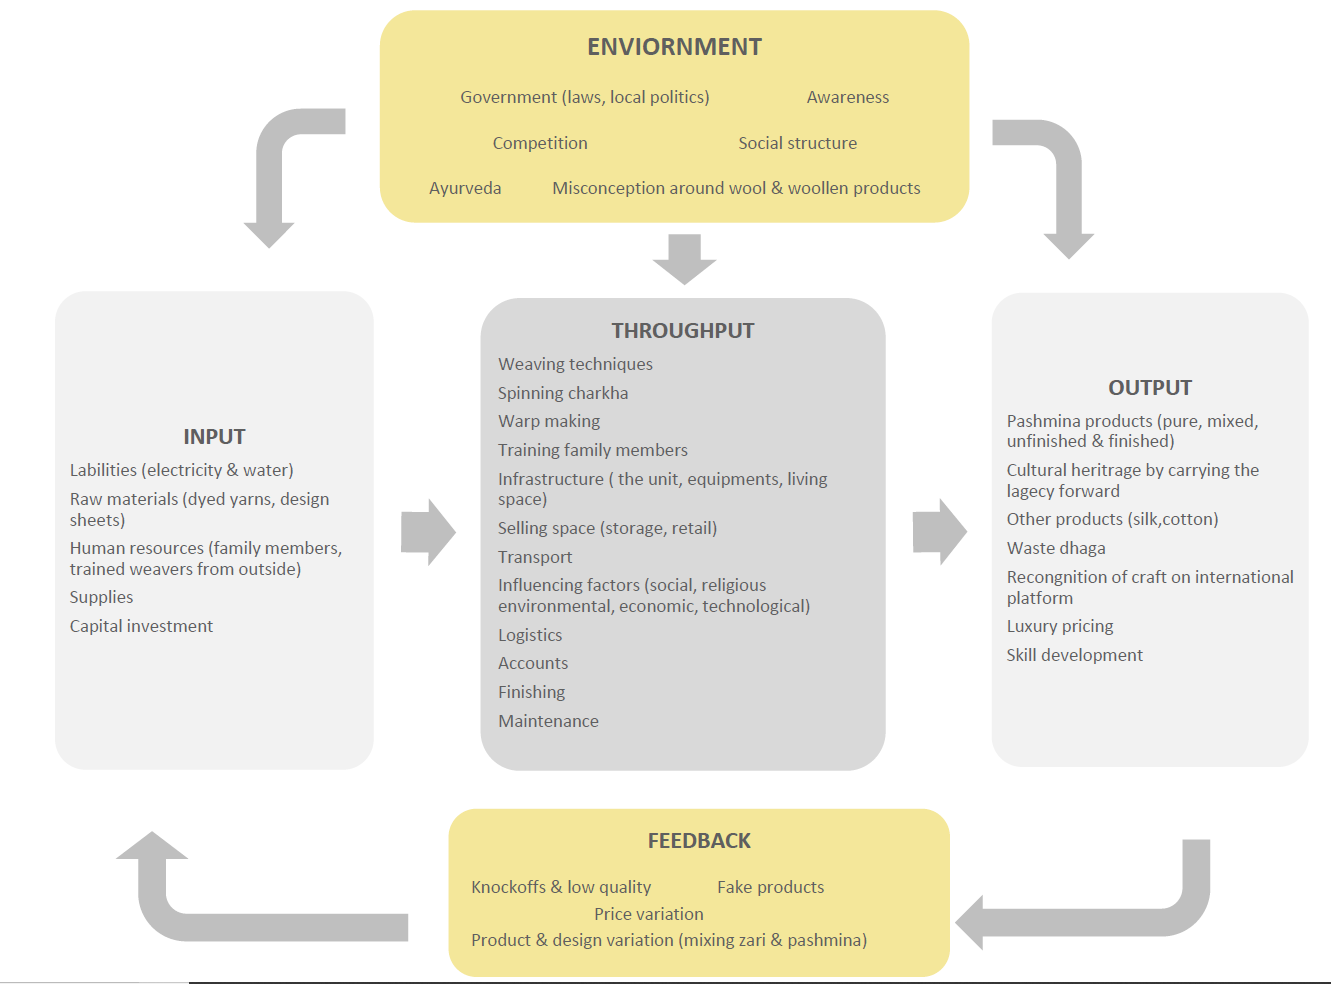
\includegraphics[width=\linewidth]{1.PNG}
  \caption{Mapping the System at the Pashmina Weaving Unit }
  \label{Existing System Map at the Pashmina Weaving Unit}
\end{figure}


\section{Effect on a Pregnant Woman's Health}
\subsection{Fibre Pollution- Wool and Pashmina} 
Wool, and Pashmina fibres being natural fibres do not have direct adverse effects on pregnancy. According to a study that was conducted to investigate possible associations between miscarriage and occupational exposures in the Shanghai Textile Industry, an elevated risk of miscarriage was found in women with exposure to synthetic fibers and a mix of synthetic and natural fibers. No elevations in risk were identified with exposure to cotton dust, endotoxin, or solvents.The suspended fibres might move deep into the lungs and affect the cardiovascular and pulmonary systems of a pregnant woman. In fact, if she is constantly exposed to such air, she may experience preterm birth (or, premature birth).

\subsection{Problems due to incorrect Posture}
Frequent crouching is associated with elevated risk of miscarriage.
There is reduced miscarriage risks associated with light to moderate occupational physical activity, and an elevated risk for women working in jobs that required crouching. Elevations in miscarriage risk associated with postural effects may be due to increases in intra-abdominal pressure, leading to decreased blood flow to the fetus. The women at the Pashmina Weaving Cluster work on \textit{charkhas} which are perched on the floor and therefore, the women are required to crouch repeatedly while working on the same. To avoid this, the \textit{charkha} could be perched on an elevated platform. This will not only help during the time of pregnancy, but it will help in maintaining the posture and reduce issues related to back pain.


\section{Possible Solutions and Future Work}

The paper deals with the various unsustainable issues that we came across in the \textit{Pashmina} Weaving unit at Shankarpur village. We've mapped issues related to the adverse effect on vision, owing to the scarcity of light, back and joint related issues due to incorrect posture, paucity of time dedicated to kids, a lack of fundamental sanitation, fibre pollution as a result of carding, and the effects on a pregnant woman's health owing mostly to incorrect posture and fiber pollution. We've mapped the system existing at the weaving unit, and have noted that most of the existing problems could be solved by the presence of a roster, clearly defining roles, and slots so that the artisans waste no time in getting redundant activities done. Another issue of sanitation could be accomplished with a better drainage system being brought into place so there is no clogging related issues. Of course, some infrastructural issues with the toilet, like the presence of a door, and a small window with a propeller would also help. 

\par
Some of the preventive measures with respect to the breathing related problems are as follows:

\begin{itemize}
    \item Wear protective gears while working in the unit. masks should be used so that the fibres are not inhaled. Respirators protect workers against insufficient oxygen environments, harmful dusts, fogs, smokes, mists, gases, vapors, and sprays. Respirators protect the user in two basic ways. The first is by the removal of contaminants from the air. Respirators of this type include particulate respirators, which filter out airborne particles, and air-purifying respirators with cartridges/canisters which filter out chemicals and gases.
    \item The unit should have proper ventilation and cross ventilation so that the workers are in contact with fresh air. Ventilation for improving or maintaining the quality of the air in the occupational work environment. Broadly defined, ventilation is a method of controlling the environment with air flow.
    \item Long term exposure to the environment where fibres could be inhaled should be avoided. Since the fibres cannot be cleaned with naked eyes, vacuum suction exhausts should be installed in work units.
    

\end{itemize}

\par
Through an interview we conducted with a former employee of Art India Export House in Jaipur, we came across the positive effects of \textit{jaggery} on the health of the employees working at the Export House. Jaggery in fact removes toxins inside one's body. Allergies caused by cough, and cold especially during winters could be dealt with by eating only 4-5 grams of jaggery, given it has anti-allergic properties. Jaggery also purifies blood, in fact post detoxification the blood flow gets improved. Since the respiratory tract is cleaned, one becomes resistive to infections as well. 

\par
Jaggery is rich in iron, and folate contents, and therefore helps in maintaining normal levels of red blood cells in one's body. It also helps in prevention of anemia. Consumption of jaggery is also very helpful for pregnant women, since it contains huge amounts of minerals and vitamins. It can also help one regain lost energy, and therefore enhance one's efficiency.  

\par
Jaggery consumed along with sesame seeds is an incredible boon. Respiratory problems ranging from bronchitis to asthma can be cured if jaggery is consumed at regular intervals with sesame seeds. Given the respiratory tract is cleared, the functioning of kidney and lungs are also regulated.


\section{References:}

A study of the occupational health function among female textile workers, 2011' \\
AJES SIAN JOURNAL OF ENVIRONMENTAL SCIENCE VOLUME 8 | ISSUE 1 | JUNE, 2013 | 64-66\\

 \url{https://search.cdc.gov/search/?query=Byssinosis&sitelimit=&utf8=%E2%9C%93&affiliate=cdc-main | Accessed 4the of April 2019}\\
 
 \url{https://www.ncbi.nlm.nih.gov/pmc/articles/PMC2862777/ | Accessed 17the of April 2019}\\
 
 \url{https://www.osha.gov/SLTC/respiratoryprotection/index.html} | Accessed 9the of April 2019\\


'Pashmina fibre —Production, characteristics and utilization'-\\
D B Shakyawa
blake@cs.stanford.edu
 A S M Raja
collinj@cs.stanford.edu
Ajay Kumar
nfm@cs.stanford.edu
P K Pareek
dabo@cs.stanford.edu
John C Mitchell
A Wani
PDF available at: https://crypto.stanford.edu/PwdHash/pwdhash.pdf \\


Kumar Mangipudi and Rajendra Katti
(Corresponding author: Kumar Mangipudi)
Department of Electrical and Computer Engineering, 1411 Centennial Blvd,
North Dakota State University, Fargo, ND 58105, USA (Email: {kumar.mangipudi, rajendra.katti}@ndsu.edu)
http://isrc.asia.edu.tw/ijns/contents/ijns-v2-n3/ijns-2006-v2-n3-p205-209.pdf\\

-\\
Pritesh N. Patel1
Jigisha K. Patel2
and Paresh V. Virparia3
Institute of Science and Technology for Advanced Studies and Research (ISTAR),
Vallabh Vidyanagar, Gujarat, India
2`I\&'3Department of Computer Science, Sardar Patel University,
Vallabh Vidyanagar, Gujarat, India
http://www.ijaiem.org/Volume2Issue6/IJAIEM-2013-06-22-060.pdf

% needed in second column of first page if using \IEEEpubid
%\IEEEpubidadjcol

% An example of a floating figure using the graphicx package.
% Note that \label must occur AFTER (or within) \caption.
% For figures, \caption should occur after the \includegraphics.
% Note that IEEEtran v1.7 and later has special internal code that
% is designed to preserve the operation of \label within \caption
% even when the captionsoff option is in effect. However, because
% of issues like this, it may be the safest practice to put all your
% \label just after \caption rather than within \caption{}.
%
% Reminder: the "draftcls" or "draftclsnofoot", not "draft", class
% option should be used if it is desired that the figures are to be
% displayed while in draft mode.
%
%\begin{figure}[!t]
%\centering
%\includegraphics[width=2.5in]{myfigure}
% where an .eps filename suffix will be assumed under latex, 
% and a .pdf suffix will be assumed for pdflatex; or what has been declared
% via \DeclareGraphicsExtensions.
%\caption{Simulation Results}
%\label{fig_sim}
%\end{figure}

% Note that IEEE typically puts floats only at the top, even when this
% results in a large percentage of a column being occupied by floats.


% An example of a double column floating figure using two subfigures.
% (The subfig.sty package must be loaded for this to work.)
% The subfigure \label commands are set within each subfloat command, the
% \label for the overall figure must come after \caption.
% \hfil must be used as a separator to get equal spacing.
% The subfigure.sty package works much the same way, except \subfigure is
% used instead of \subfloat.
%
%\begin{figure*}[!t]
%\centerline{\subfloat[Case I]\includegraphics[width=2.5in]{subfigcase1}%
%\label{fig_first_case}}
%\hfil
%\subfloat[Case II]{\includegraphics[width=2.5in]{subfigcase2}%
%\label{fig_second_case}}}
%\caption{Simulation results}
%\label{fig_sim}
%\end{figure*}
%
% Note that often IEEE papers with subfigures do not employ subfigure
% captions (using the optional argument to \subfloat), but instead will
% reference/describe all of them (a), (b), etc., within the main caption.


% An example of a floating table. Note that, for IEEE style tables, the 
% \caption command should come BEFORE the table. Table text will default to
% \footnotesize as IEEE normally uses this smaller font for tables.
% The \label must come after \caption as always.
%
%\begin{table}[!t]
%% increase table row spacing, adjust to taste
%\renewcommand{\arraystretch}{1.3}
% if using array.sty, it might be a good idea to tweak the value of
% \extrarowheight as needed to properly center the text within the cells
%\caption{An Example of a Table}
%\label{table_example}
%\centering
%% Some packages, such as MDW tools, offer better commands for making tables
%% than the plain LaTeX2e tabular which is used here.
%\begin{tabular}{|c||c|}
%\hline
%One & Two\\
%\hline
%Three & Four\\
%\hline
%\end{tabular}
%\end{table}


% Note that IEEE does not put floats in the very first column - or typically
% anywhere on the first page for that matter. Also, in-text middle ("here")
% positioning is not used. Most IEEE journals use top floats exclusively.
% Note that, LaTeX2e, unlike IEEE journals, places footnotes above bottom
% floats. This can be corrected via the \fnbelowfloat command of the
% stfloats package.



\end{document}